\documentclass[a4paper,12pt]{article}
\usepackage[T2A]{fontenc}
\usepackage[utf8x]{inputenc}
\usepackage[english,russian]{babel}
\usepackage{amsmath,amssymb,amsfonts}


\setlength{\textwidth}{16cm}
\setlength{\textheight}{25cm}
\renewcommand\baselinestretch{1.25}
\topmargin=\paperheight
\advance\topmargin-\headheight
\advance\topmargin-\headsep
\advance\topmargin-\textheight
\advance\topmargin-\footskip
\topmargin=.5\topmargin
\advance\topmargin-1truein
\oddsidemargin=\paperwidth
\advance\oddsidemargin-\textwidth
\oddsidemargin=0.5\oddsidemargin
\advance\oddsidemargin-1truein
\evensidemargin=\oddsidemargin
\tolerance1000
\emergencystretch2em

\usepackage[labelfont=bf,labelsep=period]{caption}
\usepackage{subfig}
\usepackage{pgfmath}
\usepackage{tikz}
\usetikzlibrary{arrows,fit,positioning,shapes.multipart}

\begin{document}
	\thispagestyle{empty}
% 	\centering
% 	\begin{tikzpicture}[>=latex',thick, scale=1.2, domain=0:4]
% 		\draw[draw=gray!10,fill=gray!10] (0,0) -- (.5,3) -- (6.1,3) -- (6.1,0) -- cycle;
% 		\draw[draw=gray!20,fill=gray!20] (0,0) -- (1,2) -- (6.1,2) -- (6.1,0) -- cycle;
% 		\node[below] at (1.5,3) {TVD \(\gamma=\frac1{3}\)};
% 		\node[above] at (1,0) {TVD \(\forall\gamma\)};
% 		\draw[<->] (6.3,0) node[right] {\(\theta\)} -- (0,0) -- (0,3.5) node[above] {\(\varphi(\theta)\)};
% 		\foreach \x in {0,1,2,3,4,5,6}
% 			\draw (\x cm,1pt) -- (\x cm,-1pt) node[anchor=north] {\(\x\)};
% 		\foreach \y in {0,1,2,3}
% 			\draw (1pt,\y cm) -- (-1pt,\y cm) node[anchor=east] {\(\y\)};
% 		\node[draw,circle,minimum size=.3cm] (sec) at (1,1) {};
% 		\node[text width=1.7cm,text centered] (cap) at (3,.8) {второй порядок};
% 		\draw[->] (cap.west) to (sec);
% 
% 		\draw[color=red] (0,0) -- (.1666,1) -- (1,1) -- (3,3) -- (4,3) node[above] {\textit{wide superbee} (\(\gamma=\frac1{3}\))} -- (6,3);
% 		\draw[color=blue,dashed] (0,0) -- (.1,.6) -- (3,1.888) node[below right] {\textit{wide third} (\(\gamma=\frac1{3}\))} -- (5.5,3) -- (6,3);
% 		\draw[color=green!50!black,dotted] (0,0) -- (0.333,0.667) -- (3,2) -- (5,2) node[above right] {\textit{MC}} -- (6,2);
% 	\end{tikzpicture}

\renewcommand{\thesubfigure}{\asbuk{subfigure}}

\begin{figure}
	\subfloat[схема первого порядка]{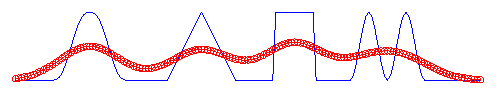
\includegraphics[width=0.5\textwidth]{conver/first}}
	\subfloat[схема Лакса"--~Вендроффа]{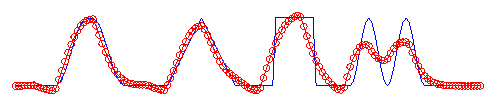
\includegraphics[width=0.5\textwidth]{conver/lax}}\\
	\subfloat[ограничитель \textit{superbee}]{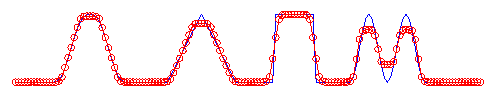
\includegraphics[width=0.5\textwidth]{conver/superbee}}
	\subfloat[ограничитель \textit{MC}]{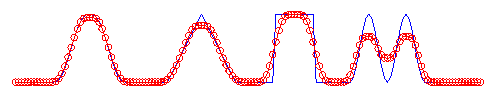
\includegraphics[width=0.5\textwidth]{conver/mc}}\\
	\subfloat[ограничитель \textit{wide superbee}]{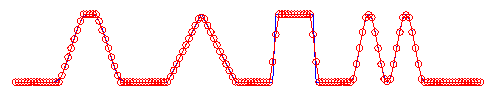
\includegraphics[width=0.5\textwidth]{conver/wide_superbee}}
	\subfloat[ограничитель \textit{wide third}]{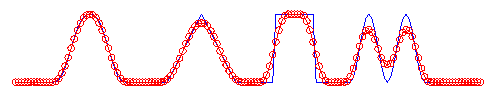
\includegraphics[width=0.5\textwidth]{conver/wide_third}}\\
\end{figure}

\end{document}
